\documentclass[10pt, twoside]{report}
\usepackage{xr}
\usepackage{listings}
\usepackage[utf8]{inputenc}
\usepackage{graphicx}
\graphicspath{ {images/} }
\usepackage{caption}
\usepackage{subcaption}
\usepackage[a4paper,width=150mm,top=25mm,bottom=25mm,bindingoffset=6mm]{geometry}

%header and footer
\usepackage{fancyhdr}
\pagestyle{fancy}
\fancyhead{}
\fancyhead[RO]{\footnotesize \leftmark}
\fancyhead[LE]{\footnotesize \rightmark}

%for table
\usepackage{multirow}

%for rotating table 
\usepackage{pdflscape}
\usepackage{rotating}

%for long table (span more than 1 page)
\usepackage{longtable}

%ASOC related paper 
\usepackage{amsmath}
\usepackage{amssymb}
\usepackage{fixltx2e}
\usepackage{diagbox}
\usepackage{makecell}
\usepackage{algorithm,algpseudocode}
\usepackage[flushleft]{threeparttable}
\usepackage{booktabs}
\usepackage{multirow}
%\usepackage{colortbl}
\usepackage[table, xcdraw]{xcolor}
\xdefinecolor{gray95}{gray}{0.45}
\xdefinecolor{gray25}{gray}{0.85}
\xdefinecolor{gray50}{gray}{0.65}
\usepackage{todonotes}
\PassOptionsToPackage{hyphens}{url}\usepackage{hyperref}
\usepackage{epstopdf}
\usepackage[normalem]{ulem}
\usepackage{amsmath} \DeclareMathOperator*{\argmax}{\arg\!\max} \DeclareMathOperator*{\argmin}{\arg\!\min}

%Nomenclature
\usepackage{nomencl}
\makenomenclature

%appendix
\usepackage[toc,page]{appendix}

\makeindex

%\usepackage[table,xcdraw]{xcolor}
%to write euro symbol
\usepackage{eurosym}

%use for subsubsection
\setcounter{secnumdepth}{3}



\usepackage{amsthm}
\theoremstyle{definition}
\newtheorem{definition}{Definition}
%ASOC related paper 


\usepackage{enumitem}

\usepackage[numbers]{natbib}


\title{
	{Ahsanullah University of Science and Technology}\\
	{\large Department of Computer Science and Engineering}\\
	{
\includegraphics{figures/AUST_logo2.png}
	}\\
	{\textbf{``BIPONEE"-An E-Commerce Web Application }
	}
	}


\author{Md. Toufiqul Islam 15.02.04.097\\
Susmoy Chakraborty  15.02.04.114\\
Nigar Sultana 15.01.04.002\\
Ovi Nazmul 13.02.04.081
}

\date{23 October 2018}


\begin{document}


\maketitle
\pagenumbering{roman}




\tableofcontents
\listoffigures
\listoftables

\clearpage
\pagenumbering{arabic}

\chapter{Introduction}


\section*{}
Now a days E-commerce website is very popular in our country. It enables the customers to choose a product or service of their choice from anywhere in the country or the world. Online shops gives us the opportunity to shop 24x7 easily. Just a couple of clicks of the mouse, we can purchase shopping products very easily, which also saves our time. Besides, online shopping allows us to find many products that user wouldn't be able to find in a physical store.\\
Our project named ``Biponee" is an E-Commerce store where there is a vast option of clothing, footwear, jewelry, accessories, electronics, appliance, books, restaurants, health & beauty products etc. We are making this project for an online shop who are currently serving their service by a Facebook page only.\\
%\section{Motivation}


%\label{sec:motivation}  

\section{Project Goal}
The goal of our project is to make it easier to sell product. Customer tracking, online payment system, customer log-in, order management, chatting with customer, cart system, efficient checkout system, promo code system, searching product is the key features of our project.\\
In addition there will be a section in our project where the admins can see the monthly buy and sell report of their shop.
\label{sec:pgoal}



\section{ Project Feasibility Analysis}
  %Feasibilit
  
  \subsection{Technical Feasibility}
  \begin{itemize}
  \item Cost of computers, laptops, printers etc.
  \item Cost of domain, hosting.
  \item Internet quality, availability of internet.
  \item Cost of internet.
  \item 24x7 availability.
  %\newpage
\end{itemize}
%\newpage

  \subsection{Operational Feasibility}
  \begin{itemize}
  \item User Friendly GUI.
  \item Tracking the product.
  \item Monthly buy and sell report.
  \item Chatting system.
  \newpage
  \item Easily add or delete product.
  \end{itemize}
 
   \subsection{ Economical Feasibility}
  \begin{itemize}
  \item Cost of Developers, Programmers etc.
  \item Cost of training the workers to operate with the system.
  \item Cost of Employee for product delivery.
  \end{itemize}
  
   \section{Cost benefit analysis}

 Tangible cost is a quantifiable cost related to an identifiable source or asset. It can be directly connected to a material item used to conduct operations or run any business. Besides  intangible cost is an unquantifiable cost relating to an identifiable source. Intangible costs represent a variety of expenses such as losses in productivity, customer goodwill, loss of brand value or damage to corporate reputation.\\
 \break
 Tangible benefits are those measured in monetary terms and intangible benefits can not be measured in monetary terms but they do have a very significant business impact. 
  
  \begin{table}[h]
  \begin{center}

\begin{tabular}{ |p{5cm}|p{5cm}|p{5cm}|  }

 \hline
  &\textbf{Cost}&\textbf{Benefit}\\
 \hline
\textbf{Tangible}  &-Direct Project Cost &-Making Product order and delivery faster\\
           &-Staff and office space&-Lower inventory cost\\
           &-Implementation Cost&-Improve the rate of productivity\\
           &&-Revenues from advertisers\\
           &&-Improved stock control\\
\hline
\textbf{Intangible}   &-Loss due to server maintenance &-Getting huge number of customers\\
             &-Loss due to training the new employees&-Online payment system\\
             &&-Customer product tracking\\
             &&-Improve Customer satisfaction\\
             &&-Graphical representation of monthly sales report\\
             &&-Improved production scheduling\\
             &&-Rating, 00comment system for customer\\
 \hline

\end{tabular}
\end{center}
\caption{Cost benefit analysis}

%\label{table1}

\end{table}

\newpage

\section{Cash-flow analysis}
Cash flow is the net amount of cash and cash-equivalents being transferred into and out of a business. It is the difference between revenue and total cost of a company. The cash flow analysis is given below:

  \begin{table}[h]
  \begin{center}


\begin{tabular}{ |p{4cm}|p{2.5cm}|p{2.5cm}|p{2.5cm} |p{2.7cm}| }
 \hline
 \multicolumn{5}{|c|}{\textbf{Year 2018}} \\
 \hline
 & \textbf{ Jun-Jul } &   \textbf {Aug-Sept} & \textbf  {Oct-Nov} & \textbf { Dec-Jan }\\
 \hline
 Revenue & 145000 & 232000 & 257000 & 294000\\
 \hline
 Costs &  &  &  & \\
 \hline
 Software Development Cost & 10000  & 10000  & 0 &0 \\
 \hline
 
 Training & 30000  & 35000  & 45000  & 52000 \\
 \hline
 Equipments &  130000 & 150000  & 110000  &  115000\\
 \hline
 Maintain & 0 &  50000 & 82000 & 92000 \\
 \hline
 Total Cost & 170000 & 245000 & 237000  & 259000 \\
 \hline
 Cash Flow & -25000 & -13000  & 20000  & 35000 \\
 \hline
Cumulative Cash Flow & -25000 & -38000  & -18000  & 17000 \\
 \hline
\end{tabular}
\end{center}
\caption{Cash-flow analysis}



\end{table}

\section{Present Value Analysis}
We know that,
\[ P.V=\frac{F.V}{(1+i)^n} \] 

\section*{}
Here,\\
P.V = Present value\\
F.V = Future value\\
i = Interest rate\\
n = Time or period\\
\\
Let us assume that for our project,\\
P.V = 20000\\
n = 4\\
i =0.08\\
So,
\[ F.V={P.V}*{(1+i)^n} \]\\ 
\[ F.V={20000}*{(1+0.08)^4} \]\\ 
\[ F.V=27210 \]\\ 
\newpage

\section{Project Scheduling}
 Project scheduling is a mechanism to communicate what tasks need to get done and which organizational resources will be allocated to complete those tasks in what timeframe. A project schedule is a document collecting all the work needed to deliver the project on time. Our project scheduling is given below: \\
 
 
 \begin{table}[h]
  \begin{center}


\begin{tabular}{ |p{2cm}|p{5cm}|p{3cm}|p{3cm}| }
 \hline
 \textbf{Activity}&\textbf{Description}&\textbf{Predecessors}&\textbf{Time(Days)}\\
 \hline
    A& Project Initiation&None&10\\
 \hline
    B&Report Submission&None&1\\
 \hline
    C&Interview \& Questioning&A, B&7\\
 \hline
    D&Project Planning&C&5\\
 \hline
    E&Analyzing System Needs &C, D&12\\
 \hline
    F&Diagram Designing&E&12\\
    \hline
    G&Data Analysis&C, F&7\\
 \hline
    H&Database Designing&F, G&10\\
\hline
 I&Coding&E, G, H&28\\
 \hline
 J&Documentation&I&5\\
 \hline
K&Testing&I&8\\
\hline
 L&Bug Fixing&K&5\\
\hline
 M&Deployment \& Training&L&10\\
 \hline
\end{tabular}
\end{center}
\caption{Project Scheduling}
\end{table}


\section{Project Scheduling Chart}


\begin{figure}
 
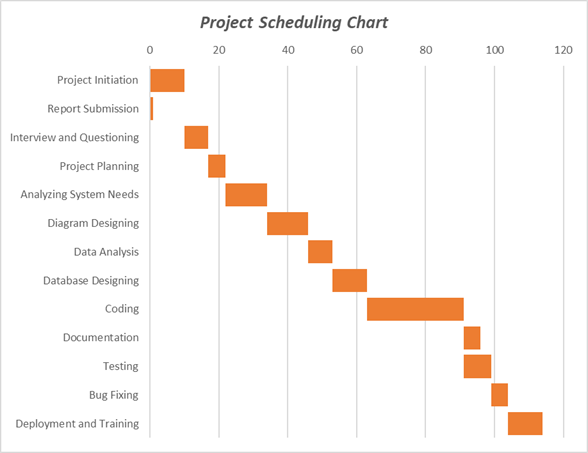
\includegraphics{figures/gantt.png}
\caption{Project Scheduling Chart}
\end{figure}

\newpage


\section{Conclusion}
 Our project ``Biponee" will take around 4 months to complete. After that we submit this project to an E-commerce company. We hope ``Biponee" will contribute a lot to the E-commerce of our country. 













 
 
 






  


\newpage
\chapter{Information Gathering}

  
\section{Selection the objectives of Information Gathering & Interview}

``Reverie Bangladesh" is a clothing (brand) which are currently selling various kinds of t-shirts through their Facebook page. After getting better response from customers and clients, they want to grow up their business.\\\\
So they offered us to develop a web based system named ``Biponee" where they can sell variety of products such as men's clothing, women's clothing, watch and jewelry, electronics etc.\\\\
So, to know about how their existing system works, how they maintain it, we called an interview on 24 May, 2018. This interview helps us to gather information from them which is helpful for us to improve features to this project.

\section{Questionnaires and Interview pattern}
To know the client requirements, we need to gather information from them. There are various way to gather information. Some of them are describing below:\\

\textbf{Interview:} An interview is a conversation where questions are asked and answers are given. Interviews usually take place face to face and in person. We can modify it. In an interview we gather information by asking questions to the interviewee. There are two types of questions, which are:\\
 
  \underline{1. Open-ended Question:} Open-ended questions are ones that require more than one word answers. “Open” actually describes the interviewee’s options for responding. They are open. The response can be two words or two paragraphs. \\\\
\underline{2. Closed Question:} Closed  questions can be answered in only one word or with a short, specific piece of information. A closed question limits the response available to the interviewee. \\
 
\textbf {Questionnaire:} A questionnaire is a research instrument consisting of a series of questions (or other types of prompts) for the purpose of gathering information from respondents. Questionnaires are also sharply limited by the fact that respondents must be able to read the questions and respond to them. In this process we can not modify the question and it is not necessary to face to face interaction.\\

For information gathering we use interview method, because for our project we need to interact with the client face to face for analyze their requirements. We used Pyramid structure for our system.


 \section{Selection of interview Personnel}
 We have selected Mr. Rahee Zaman, founder of ``Reverie Bangladesh" for the interview. For our project it is necessary to know how they currently running their system, what are the difficulties they are facing to running this system, what are the requirements and features they want in ``Biponee". As a founder of "Reverie Bangladesh", Mr. Rahee Zaman knows everything about their existing system. So the whole interview was taken from him.
 
  \section{Summary of the total information and list of activities}
  After interviewing Mr. Rahee Zaman, we identify the drawbacks of their current system. We also know about some new features we need to integrate in ``Biponee". Besides they shared with us about the difficulties they are facing right now and about the future plan of Reverie Bangladesh.  \\
  
  The list of activities   are:
  \begin{itemize}
  \item Knowing about order management
  \item Knowing about delivery system
  \item Current payment system
  \item Current inventory management
  \item  Reasons behind shifting to BIPONEE
   \item Features 
   \item Future plan
\end{itemize}

\section{Conclusion}
After the information gathering process, we have a complete idea  about how they manage their sections, what they want in ``Biponee", how they take/serve the orders from/to the customer, communicate with the customer etc. Hopefully by our project ``Biponee" they will manage their business smartly, will achieve customer satisfaction, and grow up their business rapidly.
  
  
  
 
 






\chapter{Data Flow Diagram and Use case Diagram}


\section{Data Flow Diagram}

A data flow diagram (DFD) is a graphical representation of the "flow" of data through an information system, modelling its process aspects. A DFD is often used as a preliminary step to create an overview of the system without going into great detail, which can later be elaborated.
\subection{Activities of the project}
\begin{itemize}
  \item Login/Sign up
  \item Browse sections
    \item Cart system
  \item Product tracking
  
\end{itemize}


 \subsection{Main Process}
 
 \begin{itemize}
  \item Biponee - An online shopping system
  \end{itemize}

 \subsection{Sub-process}
  \begin{itemize}
    \item Sign up
    \item Login
    \item Edit section
    \item Edit products
    \item Search products
    \item Add to cart
    \item Checkout
     \item View orders
    \item Show customers information
    \item Product tracking
    \item Analysis
    
    

\end{itemize}


\subsection{Entity  }
  \begin{itemize}
  \item Customer
  \item Visitor
    \item Admin
  
    
    

\end{itemize}
\subsection{Data store}
  \begin{itemize}
  \item Customers
  \item Admins
    \item Carts
  \item Orders
  \item Products
    \item Sections
  
\end{itemize}

\subsection{Levels of Data Flow Diagram}
  \begin{itemize}
  \item Context level DFD
  \item Level 1 DFD
    \item Level 2 DFD
  
  
\end{itemize}



\subsection{Context level DFD}
A context diagram is a top level (also known as ``Level 0") data flow diagram. It only contains one process node (``Process 0") that generalizes the function of the entire system in relationship to external entities.\\

 \begin{figure}
 \centering
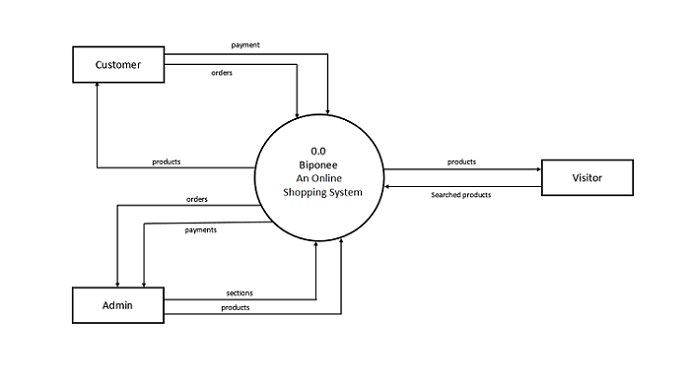
\includegraphics{figures/level0final.png}
\caption{Context Level DFD of Biponee}
\end{figure}

\newpage

\subsection{level 1 DFD}
 \begin{figure}
 \centering
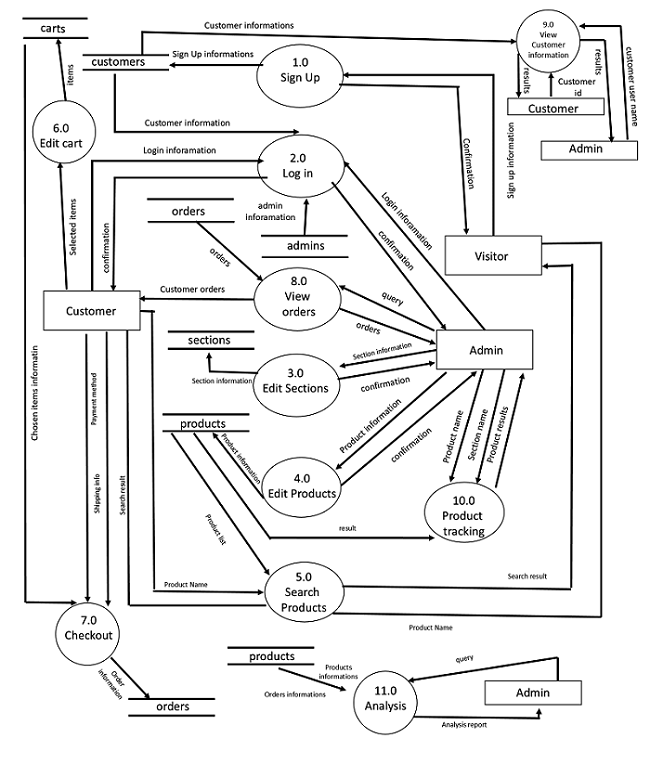
\includegraphics{figures/1s.png}
\caption{Level 1 DFD of Biponee}
\end{figure}


\newpage

\subsection{ Level 2 DFD }
 \begin{figure}
 \centering
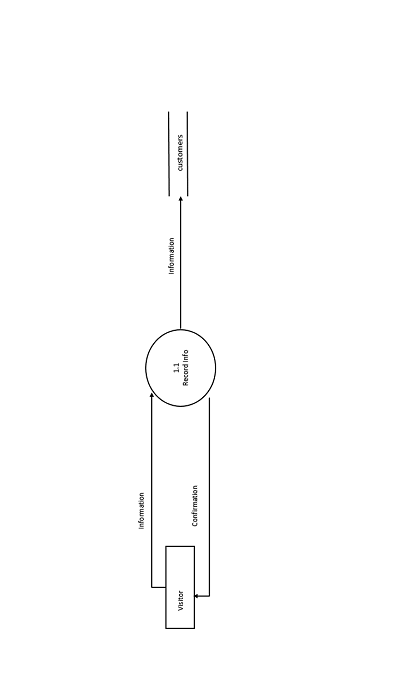
\includegraphics{figures/1final.png}
\caption{Sub-processes of Sign Up}
\end{figure}






 \begin{figure}
 \centering
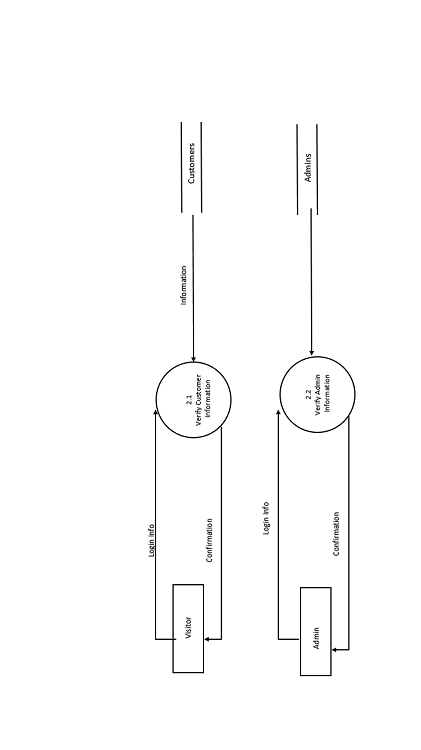
\includegraphics{figures/2final.png}
\caption{Sub-processes of Log in}
\end{figure}


 \begin{figure}
 \centering
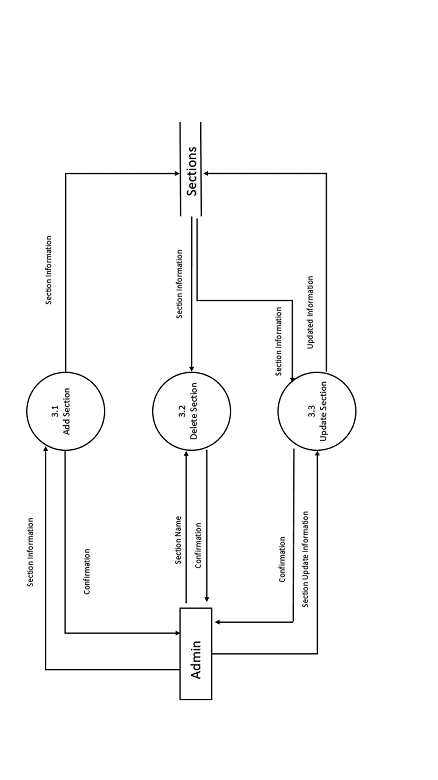
\includegraphics{figures/3final.png}
\caption{Sub-processes of Edit Sections}
\end{figure}



 \begin{figure}
 \centering
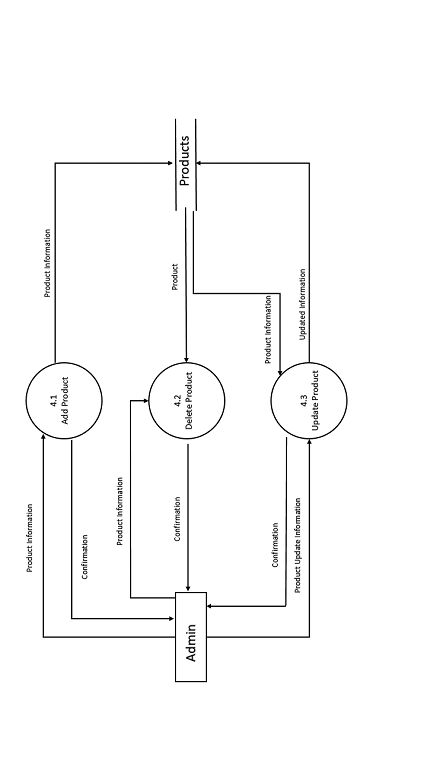
\includegraphics{figures/4final.png}
\caption{Sub-processes of Edit products}
\end{figure}



\begin{figure}
 \centering
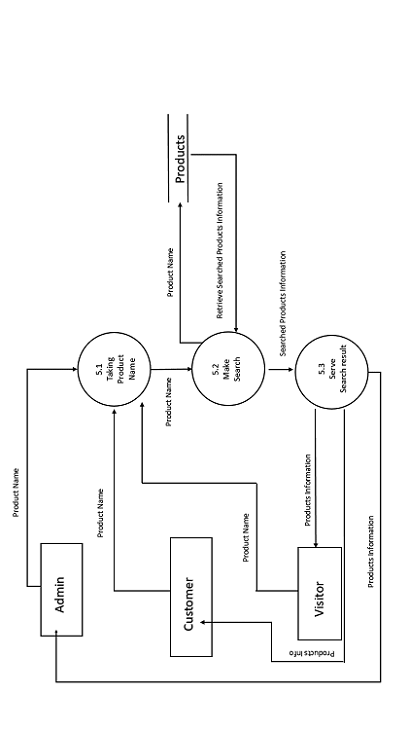
\includegraphics{figures/5final.png}
\caption{Sub-processes of Search Products}
\end{figure}




\begin{figure}
 \centering
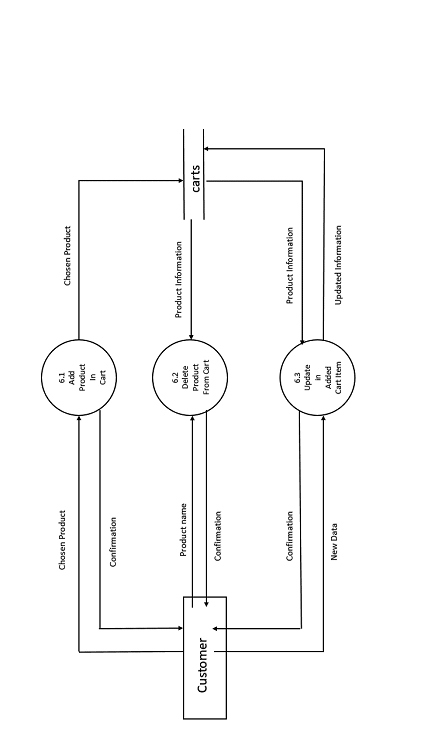
\includegraphics{figures/6final.png}
\caption{Sub-processes of  Edit cart}
\end{figure}


\begin{figure}
 \centering
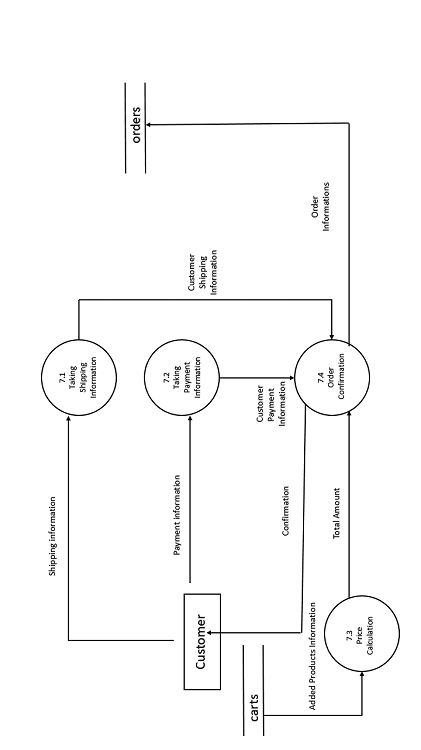
\includegraphics{figures/7final.png}
\caption{Sub-processes of  Order confirmation}
\end{figure}

\begin{figure}
 \centering
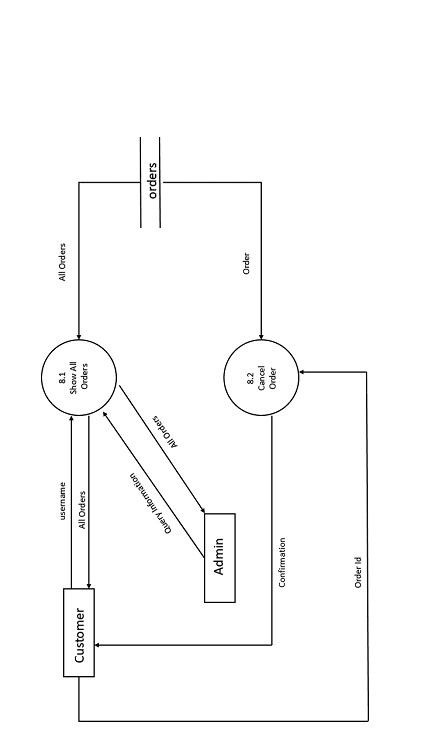
\includegraphics{figures/8final.png}
\caption{Sub-processes of View orders}
\end{figure}



\begin{figure}
 \centering
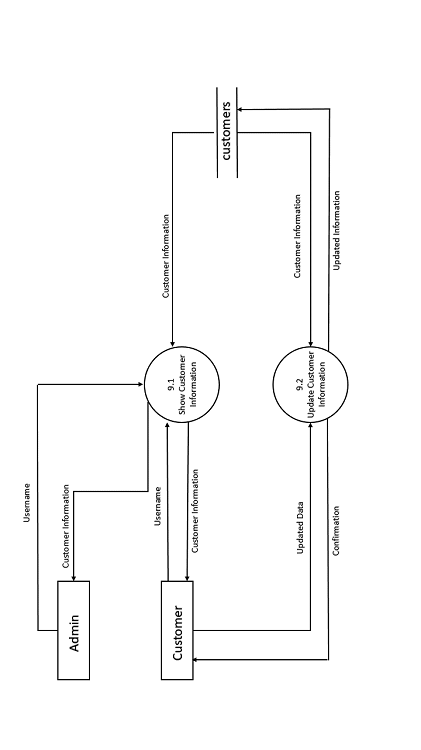
\includegraphics{figures/9final.png}
\caption{Sub-processes of View Customer information}
\end{figure}




\begin{figure}
 \centering
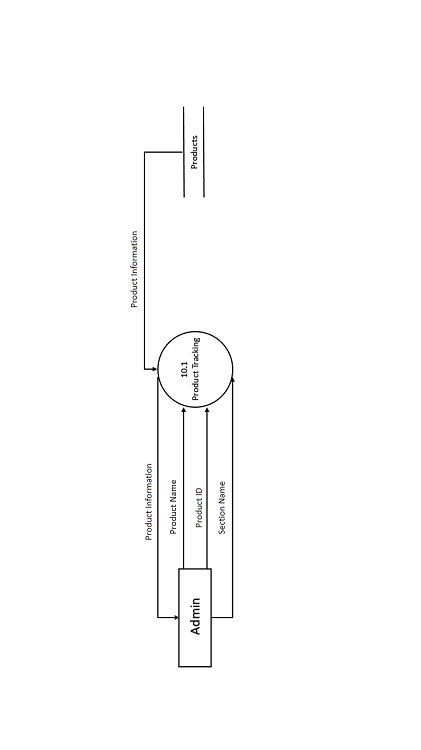
\includegraphics{figures/10final.png}
\caption{Sub-processes of Product tracking}
\end{figure}



\begin{figure}
 \centering
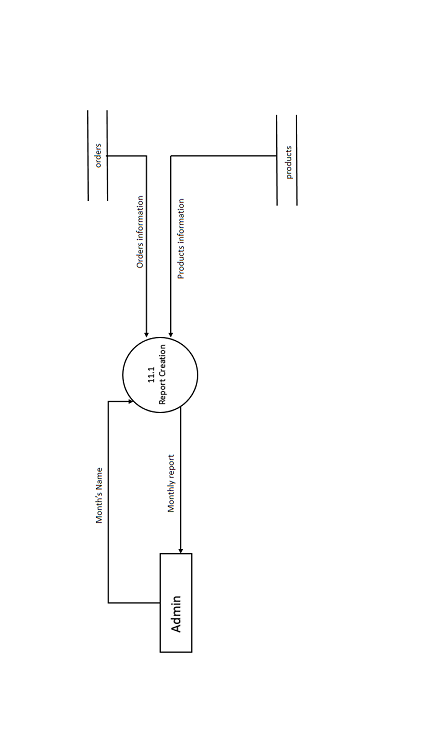
\includegraphics{figures/11final.png}
\caption{Sub-processes of Analysis}
\end{figure}

\newpage
\section{ Use Case Diagram}
 A use case diagram at its simplest is a representation of a user's interaction with the system that shows the relationship between the user and the different use cases in which the user is involved.
 
 \subsection{Actors}
  An actor specifies a role played by a user or any other system that interacts with the subject.\\ 
  The list of actors used by us:
\begin{itemize}
  \item Customer
  \item Visitor
    \item Admin
  \item Biponee Website
\end{itemize}


\subsection{Use Cases}
Use case is the sequence of actions that the system performs that yields an
observable result of value to an actor.
\begin{itemize}
  \item Sign up
  \item Login
    \item Browse sections
  \item Add to cart
    \item Checkout
  \item Edit sections
    \item Edit products
    \item View orders
    \item View customer informations
    \item Product tracking
    \item Analysis
    \item Confirmation
    \item Verify password
    \item Display login error
    \item Total calculation
    \item Update sections table
    \item Update products table
    \item Report calculations
 
\end{itemize}


\newpage
\subsection{Details of Use Case Models}

 \begin{figure}
\centering

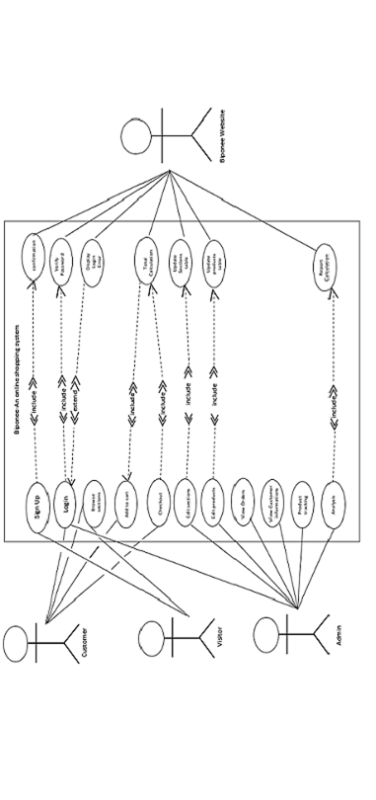
\includegraphics{figures/usecasenewv.png}

\caption{Use Case Diagram of Biponee}
\end{figure}


\newpage
\subsection{Conclusion}
 \begin{itemize}
    A Data flow diagram shows what kind of information will be input to and output from the system, how the data will advance through the system, and where the data will be stored. It does not show informations about process timing. From the DFD we can gather the clear concept of data flow of our project.\\
    \\
    
    We also draw the use case diagram of Biponee. we identify the actors and the use cases of our project from the diagram. We also identify how actually the actors communicate with the use cases from this diagram.\\
    \\
    
    We hope this use case diagram and data flow diagram concept will help us for develop Biponee
    efficiently.\\
     
 \end{itemize}


\chapter{Entity Relationship Diagram and Class Diagram}
\section{Entity-Relationship Diagram}
An entity relationship diagram (ERD), also known as an entity relationship model, is a graphical representation of an information system that depicts the relationships among people, objects, places, concepts or events within that system. An ERD is a data modeling technique that can help define business processes and be used as the foundation for a relational database.\\
\subsection{Entity}
\begin{itemize}
\item Admin
\item User
\item Section
\item Products
\item Cart
\item Orders

\end{itemize}
\subsection{Attribute}
\begin{itemize}

\item Admin: AdminID, FirstName, LastName, Password
\item User: Email, FirstName, LastName, Password, UserID 
\item Section: SectionID, SectionName
\item Products: Quantity, Sizes, Description, Category, Price, SectionID, ProductCode, ProductName, ProductID, ImgLink, Bandname

\item Cart: Quantity, UserID, OrderID, ProductID, SubTotal, CartItemID
\item Orders: orderID, FirstName, PaymentMethod, Total, CartItemID, UserID, Adress, Phone, LastName 


\end{itemize}



 \subsection{Relationship}
 \begin{itemize}
  \item Admin manages Order
  \item Section contains product
  \item Cart contain product
  \item Order contains cart
  \item User places order

    \end{itemize}
   \subsection{Diagram}
   
   \begin{figure}
 \centering
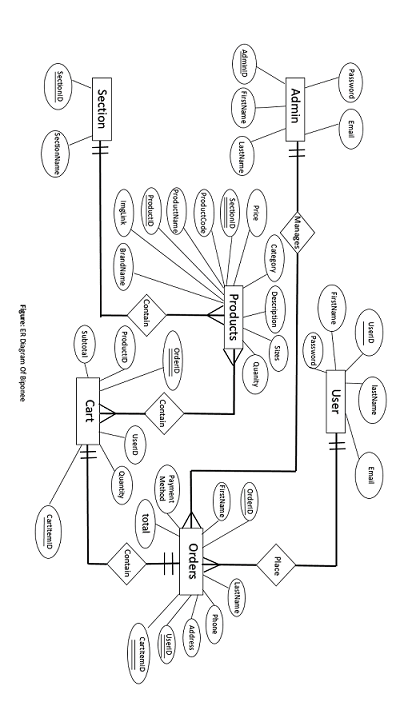
\includegraphics{figures/erdplus.png}
\caption{ERD of Biponee}
\end{figure}


\newpage

\section{Class Diagram}
Class diagrams are one of the most useful types of diagrams in UML as they clearly map out the structure of a particular system by modeling its classes, attributes, operations, and relationships between objects.\\


\subsection{Class}
\begin{itemize}
    \item User
    \item Admin
    \item ClothingsProduct
    \item Section
    \item Order
    \item Product
    \item CartItem
     \item OthersProduct
    
\end{itemize}


\subsection{Relationship}

\begin{itemize}
    \item Inheritance
    \item Association
    \item Aggregation
    \item Composition  
\end{itemize}
  
  
 \subsection{Multiplicity}
 \begin{itemize}
     \item 0 to 1 (Zero to one)
     \item 0...* (Zero to many) 
     \item 1...* (One to many)
     \item m...n (Specific number range)
     
 \end{itemize}
  \subsection{Diagram}
  \begin{figure}
 \centering
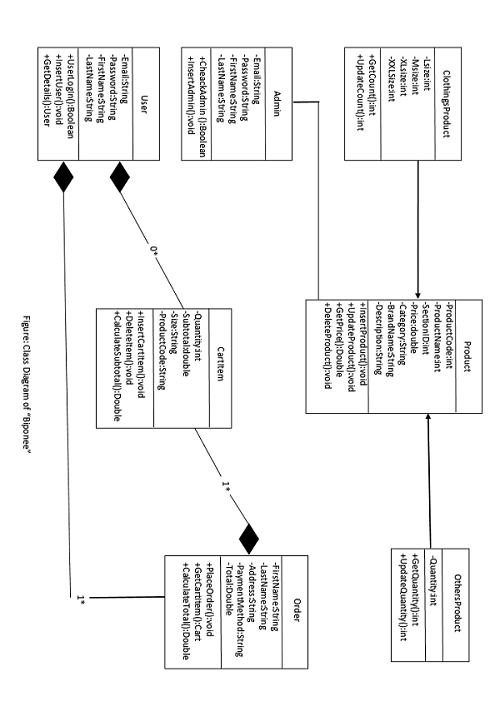
\includegraphics{figures/classfinal.png}
\caption{Class Diagram of Biponee}
\end{figure}


\newpage

\section{Conclusion}
 Entity relationship diagrams provide a visual starting point for database design that can also be used to help determine information system requirements throughout an organization. After a relational database is rolled out, an ERD can still serve as a referral point, should any debugging or business process re-engineering be needed later. We draw our ER Diagram which give us the clear Reflection of our project database.\\
 In Class Diagram a class defines the methods and variables in an object, which is a specific entity in a program or the unit of code representing that entity. Class diagrams are useful in all forms of object-oriented programming (OOP). 

\chapter{Discussion}
For developing ‘Biponee’ we follow different phases.At first we analyze the project feasibility. Here we analyze three kinds of project feasibility. They are operational feasibility, technical feasibility and economical feasibility. \\
After that we analyze cost benefit and present value and future value of the project finally we make a project scheduling chart at this step.\\
Then we go to information gathering phase. In this phase we collect information from our client “Reverie Bangladesh” and gain the complete idea about how they manage their current system. \\
In the next step we design the data flow diagram and Use case diagram. From data flow diagram we identified what kind of data will be the input and output of our project, how data will advance in this system and where the data will be stored. From use case diagram we identify the use case and the actors of our project.\\
Then we design the ER diagram and class diagram. In ER diagram we identify the entities and relationships of our project. The ER diagram provide the visual starting point of our project database. The class diagram defines the method and variables of an object. This class diagram is useful in all forms of object oriented programming.\\\\
The technologies we used in frontend development are:
\begin{itemize}
    \item HTML
    \item CSS
    \item Javascript
    \item jQuery
    \item AJAX
\end{itemize}
\\\\
The technologies we used in backend are:
\begin{itemize}
    \item C#
    \item SQL
    
\end{itemize}
\\\\

The IDE we used in this project development:
\begin{itemize}
    \item Microsoft Visual Studio 2018
    \item Microsoft SQL Server Management Studio 17
    
\end{itemize}
\\\\

The architecture we used:
\begin{itemize}
    \item MVC Architecture
    \item Layer Architecture
    
\end{itemize}
\\\\
The framework we used:
\begin{itemize}
    \item Asp.net MVC Framework
\end{itemize}
\\
In the future we will add more section in our project. Try to implement Artificial intelligence(AI), and Machine learning to make our project more efficient. 






\begin{appendices}
  \chapter{Implementation}
  \section{Model}
\subsection{AdminC.cs}
\begin{lstlisting}
using System;
using System.Collections.Generic;
using System.Linq;
using System.Web;

namespace Biponee.Models
{
    public class AdminC
    {
        public int ID { get; set; }
        public String Email { get; set; }
        public String Password { get; set; }
        public String FirstName { get; set; }
        public String LastName { get; set; }

        public AdminC(int iD, String email, String password,
        String firstName, String lastName)
        {
            ID = iD;
            Email = email;
            Password = password;
            FirstName = firstName;
            LastName = lastName;
        }

        public AdminC(String email, String password,
        String firstName, String lastName)
        {
            Email = email;
            Password = password;
            FirstName = firstName;
            LastName = lastName;
        }

        public AdminC()
        {
        }
    }
}
\end{lstlisting}

\newpage
\subsection{UserC.cs}

\begin{lstlisting}
using System;
using System.Collections.Generic;
using System.Linq;
using System.Web;

namespace Biponee.Models
{
    public class UserC
    {
        public int Id { get; set; }
        public String FirstName { get; set; }
        public String LastName { get; set; }
        public String Email { get; set; }
        public String Password { get; set; }

        public UserC(int id, string firstName, 
        string lastName, string email, string password)
        {
            Id = id;
            FirstName = firstName;
            LastName = lastName;
            Email = email;
            Password = password;
        }

        public UserC( string firstName,string lastName, 
        string email, string password)
        {
           
            FirstName = firstName;
            LastName = lastName;
            Email = email;
            Password = password;
        }


    }
}
\end{lstlisting}
\newpage

\subsection{CartItemC.cs}
\begin{lstlisting}
using System;
using System.Collections.Generic;
using System.Linq;
using System.Web;

namespace Biponee.Models
{
    public class CartItemC
    {
        public int OrderId { get; set; }
        public int ProductId { get; set; }
        public String ProductImage { get; set; }
        public String ProductName { get; set; }
        public String ProductSize { get; set; }
        public Double UnitPrice { get; set; }
        public int Qty { get; set; }
        public Double Subtotal { get; set; }

        public CartItemC(int orderId,int productId, 
        string productImage, string productName, 
        string productSize,double unitPrice, int qty, double subtotal)
        {
            OrderId = orderId;
            ProductId = productId;
            ProductImage = productImage;
            ProductName = productName;
            ProductSize = productSize;
            UnitPrice = unitPrice;
            Qty = qty;
            Subtotal = subtotal;
        }
        public CartItemC( int productId, string productImage, 
        string productName, string productSize, 
        double unitPrice, int qty, double subtotal)
        {
            
            ProductId = productId;
            ProductImage = productImage;
            ProductName = productName;
            ProductSize = productSize;
            UnitPrice = unitPrice;
            Qty = qty;
            Subtotal = subtotal;
        }


    }
}

\end{lstlisting}
\newpage

\subsection{OrderC.cs}
\begin{lstlisting}
using System;
using System.Collections.Generic;
using System.Linq;
using System.Web;

namespace Biponee.Models
{
    public class OrderC
    {
        public int OrderId { get; set; }
        public String FirstName { get; set; }
        public String LastName { get; set; }
        public String Phone { get; set; }
        public String Address { get; set; }
        public String State { get; set; }
        public String City { get; set; }
        public int UserId { get; set; }
        public String PaymentMethod { get; set; }
        public Double Total { get; set; }

       public OrderC(int orderId, string firstName,
       string lastName, string phone,
       string address, string state,
       string city, int userId,
       string paymentMethod, double total)
        {
            OrderId = orderId;
            FirstName = firstName;
            LastName = lastName;
            Phone = phone;
            Address = address;
            State = state;
            City = city;
            UserId = userId;
            PaymentMethod = paymentMethod;
            Total = total;
        }
        public OrderC(string firstName, string lastName,
        string phone, string address,
        string state, string city, int userId, 
        string paymentMethod, double total)
        {
            FirstName = firstName;
            LastName = lastName;
            Phone = phone;
            Address = address;
            State = state;
            City = city;
            UserId = userId;
            PaymentMethod = paymentMethod;
            Total = total;
        }
    }
}
\end{lstlisting}

\newpage


\subsection {ClothingProduct.cs}
\begin{lstlisting}
using System;
using System.Collections.Generic;
using System.Linq;
using System.Web;

namespace Biponee.Models.Products
{
    public class ClothingProduct : Product
    {
        public int LCount { get; set; }
        public int MCount { get; set; }
        public int XLCount { get; set; }
        public int XXLCount { get; set; }

        public ClothingProduct(String productName,
        String productCode, int sectionId,
        Double price,String category,
        String description,
        String imageLink,String brandName,
            int lCount,int mCount,int xlCount,
            int xxlCount) 
            :base(productName,
            productCode,sectionId,price,
            category,description,imageLink,
            brandName)
        {
            this.LCount = lCount;
            this.MCount = mCount;
            this.XLCount = xlCount;
            this.XXLCount = xxlCount;
        }

        public ClothingProduct(int productId,
        String productName, String productCode, 
        int sectionId, Double price, 
        String category, 
        String description, 
        String imageLink,
        String brandName,
           int lCount, int mCount, 
           int xlCount, int xxlCount) 
           : base(productId,
           productName, 
           productCode, sectionId, price, 
           category, 
           description, imageLink, brandName)
        {
            this.LCount = lCount;
            this.MCount = mCount;
            this.XLCount = xlCount;
            this.XXLCount = xxlCount;
        }

        public ClothingProduct():base()
        {
        }
    }
}

\end{lstlisting}
\newpage

\subsection{DailyNeedProduct.cs}

\begin{lstlisting}
using System;
using System.Collections.Generic;
using System.Linq;
using System.Web;

namespace Biponee.Models.Products
{
    public class DailyNeedProduct : Product
    {
       public int Quantity { get; set; }
        public DailyNeedProduct(string productName, 
        string productCode, int sectionId,
        double price,int quntity ,string category, 
        string description, string imageLink, 
        string brandName) : base(productName, 
        productCode, sectionId, price, category, 
        description, imageLink, brandName)
        {
            this.Quantity = quntity;
        }

        public DailyNeedProduct(int id,
        string productName, string productCode, 
        int sectionId, 
        double price, int quntity, string category, 
        string description, 
        string imageLink, 
        string brandName) : base(id,productName, 
        productCode, sectionId, price, category, 
        description, imageLink, brandName)
        {
            this.Quantity = quntity;
        }

        public DailyNeedProduct() : base()
        {

        }
    }
}


\end{lstlisting}

\newpage

\subsection{ElectronicsProduct.cs}
\begin{lstlisting}
using System;
using System.Collections.Generic;
using System.Linq;
using System.Web;

namespace Biponee.Models.Products
{
    public class ElectronicsProduct : Product

    {

        public int Quantity { get; set; }
        public ElectronicsProduct(string productName, 
        string productCode, int sectionId, double price, 
        int quantity,string category,
        string description,
        string imageLink,
        string brandName) : base(productName, productCode,
        sectionId, price, category,
        description, imageLink, brandName)
        {
            this.Quantity = quantity;
        }
        public ElectronicsProduct(int id,string productName, 
        string productCode, int sectionId,
        double price, int quantity, string category, 
        string description, string imageLink, 
        string brandName) : base(id,
        productName, productCode, 
        sectionId, price, category, 
        description, imageLink, brandName)
        {
            this.Quantity = quantity;
        }

        public ElectronicsProduct():base()
        {
        }
    }
}


\end{lstlisting}

\subsection{MobileProduct.cs}
\begin{lstlisting}
using System;
using System.Collections.Generic;
using System.Linq;
using System.Web;

namespace Biponee.Models.Products
{
    public class MobileProduct : Product
    {
        public int Quantity { get; set; }
        public MobileProduct(string productName, 
        string productCode, int sectionId, 
        double price, int quantity,
        string category, string description, 
        string imageLink, string brandName) : 
        base(productName, productCode, 
        sectionId, price, category, 
        description, imageLink, brandName)
        {
            this.Quantity = quantity;
        }
        public MobileProduct(int id,string 
        productName, string productCode, 
        int sectionId, double price, 
        int quantity, string category, 
        string description, 
        string imageLink, 
        string brandName) : base(id,productName, 
        productCode, sectionId, price, category, 
        description, 
        imageLink, brandName)
        {
            this.Quantity = quantity;
        }


        public MobileProduct() : base()
        {

        }
    }
}

\end{lstlisting}

\newpage

\subsection{Product.cs}
\begin{lstlisting}
using System;
using System.Collections.Generic;
using System.Linq;
using System.Web;

namespace Biponee.Models.Products
{
    public class Product
    {
        public int ProductId { get; set; }
        public String ProductName { get; set; }
        public String ProductCode { get; set; }
        public int SectionId { get; set; }
        public Double Price { get; set; }
        public String Category { get; set; }
        public String Description { get; set; }
        public String ImageLink { get; set; }
        public String BrandName { get; set; }

        public Product(string productName, 
        string productCode, int sectionId, 
        Double price, string category, 
        string description, 
        string imageLink, string brandName)
        {
            ProductName = productName;
            ProductCode = productCode;
            SectionId = sectionId;
            Price = price;
            Category = category;
            Description = description;
            ImageLink = imageLink;
            BrandName = brandName;
        }

        public Product(int productId,
        string productName, 
        string productCode, int sectionId, 
        Double price, string category, string description, 
        string imageLink, string brandName)
        {
            ProductId = productId;
            ProductName = productName;
            ProductCode = productCode;
            SectionId = sectionId;
            Price = price;
            Category = category;
            Description = description;
            ImageLink = imageLink;
            BrandName = brandName;
        }

        public Product()
        {
        }
    }
}


\end{lstlisting}
\newpage

\section{Database}

\subsection{AdminGetway.cs}

\begin{lstlisting}

using Biponee.Models;
using System;
using System.Collections.Generic;
using System.Data.SqlClient;
using System.Linq;
using System.Web;
using System.Web.Configuration;

namespace Biponee.DLL
{
    public class AdminGetway
    {
        String connectionString = WebConfigurationManager.ConnectionStrings
        ["biponeeDbConnectioon"].ConnectionString;

        public List<AdminC> getAdminByEmailAnsPassword
        (String email, String Password)
        {
            SqlConnection connection = new 
            SqlConnection(connectionString);
            String Query = "SELECT * FROM admins
            WHERE Email = '" + email + "'
            AND Password = '" + Password + "'";

            SqlCommand command = new SqlCommand(Query, connection);
            connection.Open();
            SqlDataReader reader = command.ExecuteReader();

            List<AdminC> list = new List<AdminC>();

            while (reader.Read())
            {
                int id = Convert.ToInt32(reader["AdminID"]);
                String adminEmail = reader["Email"].ToString();
                String password = reader["Password"].ToString();
                String firstName = reader["FirstName"].ToString();
                String lastName = reader["LastName"].ToString();

               list.Add( new AdminC(id, adminEmail, password, firstName, lastName));
            }

            return list;
        }

        public List<AdminC> getAdminById(int adminId)
        {
            SqlConnection connection = new 
            SqlConnection(connectionString);
            String Query = "SELECT * FROM admins 
            WHERE AdminID = " + adminId;

            SqlCommand command = new 
            SqlCommand(Query, connection);
            connection.Open();
            SqlDataReader reader = command.ExecuteReader();

            List<AdminC> list = new List<AdminC>();

            while (reader.Read())
            {
                int id = Convert.ToInt32(reader["AdminID"]);
                String adminEmail = reader["Email"].ToString();
                String password = reader["Password"].ToString();
                String firstName = reader["FirstName"].ToString();
                String lastName = reader["LastName"].ToString();

                list.Add(new AdminC(id, adminEmail, 
                password, firstName, lastName));
            }

            return list;
        }
    }
}
\end{lstlisting}

\newpage

\subsection{OrderGetway.cs}

\begin{lstlisting}
using System;
using System.Collections.Generic;
using Biponee.Models;
using System.Web;
using System.Web.Configuration;
using System.Data.SqlClient;

namespace Biponee.DAL
{
    public class OrderGetway
    {
        String connectionString =
        WebConfigurationManager.ConnectionStrings
        ["biponeeDbConnectioon"].ConnectionString;

        public int InsertOrder(OrderC order)
        {
            SqlConnection connection = new
            SqlConnection(connectionString);
            String Query = "INSERT 
            INTO orders VALUES ('" + order.FirstName + "','" 
            + order.LastName + "','" + order.Phone + "','" + 
            order.Address + "','" + order.State + "','" +
            order.City + "'," + 
            order.UserId + ",'" + 
            order.PaymentMethod + "'," + order.Total + ")";
            SqlCommand command = new SqlCommand(Query, connection);
            connection.Open();
            int res = command.ExecuteNonQuery();
            connection.Close();

            return res;
        }
    }
}
\end{lstlisting}

\newpage

\subsection{ProductGetway.cs}

\begin{lstlisting}
using Biponee.Models;
using Biponee.Models.Products;
using System;
using System.Collections.Generic;
using System.Data.SqlClient;
using System.Linq;
using System.Web;
using System.Web.Configuration;

namespace Biponee.DLL
{
    public class ProductGetway
    {
        String connectionString = WebConfigurationManager.
        ConnectionStrings["biponeeDbConnectioon"].ConnectionString;

        public int insertClothingProduct(ClothingProduct product)
        {
            SqlConnection connection = 
            new SqlConnection(connectionString);
            String Query = "INSERT INTO products 
            VALUES ('" + product.ProductName + "','" + 
            product.ProductCode + "'," + product.SectionId + "," 
            + product.Price + ",'" + product.Category + "','" 
            + product.Description + "','" + product.ImageLink + "'," + 
            product.LCount + "," + product.MCount + "," + 
            product.XLCount + "," + product.XXLCount+",null" + ",'" + 
            product.BrandName + "')";
            SqlCommand command = new SqlCommand(Query, connection);
            connection.Open();
            int res = command.ExecuteNonQuery();
            connection.Close();

            return res;
        }

        public int insertElectronicsProduct
        (ElectronicsProduct product)
        {
            SqlConnection connection = new 
            SqlConnection(connectionString);
            String Query = "INSERT INTO products 
            VALUES ('" + 
            product.ProductName + "','" + product.ProductCode + "'," 
            + product.SectionId + "," + product.Price + ",'" 
            + product.Category + 
            "','" + product.Description + "','" + 
            product.ImageLink + "',null,null,null,null,"  + 
            product.Quantity + ",'" + product.BrandName + "')";
            SqlCommand command = new SqlCommand(Query, connection);
            connection.Open();
            int res = command.ExecuteNonQuery();
            connection.Close();

            return res;
        }

        public int insertDailyNeedsProduct
        (DailyNeedProduct product)
        {
            SqlConnection connection = new 
            SqlConnection(connectionString);
            String Query = "INSERT INTO products VALUES 
            ('" + product.ProductName + "','" + 
            product.ProductCode + "'," + product.SectionId + "," + 
            product.Price + ",'" + product.Category + "','" + 
            product.Description + "','" + product.ImageLink + "',
            null,null,null,null," + product.Quantity + ",'" +
            product.BrandName + "')";
            SqlCommand command = new 
            SqlCommand(Query, connection);
            connection.Open();
            int res = command.ExecuteNonQuery();
            connection.Close();

            return res;
        }
        public int insertMobileProduct
        (MobileProduct product)
        {
            SqlConnection connection = new 
            SqlConnection(connectionString);
            String Query = "INSERT INTO products VALUES 
            ('" + product.ProductName + "','" + product.ProductCode 
            + "'," + product.SectionId + "," + product.Price + ",'" 
            + product.Category + 
            "','" + product.Description + "','" 
            + product.ImageLink + "',
            null,null,null,null," 
            + product.Quantity + ",'" + 
            product.BrandName + "')";
            SqlCommand command = new SqlCommand
            (Query, connection);
            connection.Open();
            int res = command.ExecuteNonQuery();
            connection.Close();

            return res;
        }


        public List<ClothingProduct> getAllClothingProduct()
        {
            SqlConnection connection =
            new SqlConnection(connectionString);
            String Query = "SELECT * FROM products 
            WHERE SectionId = 1";

            SqlCommand command = new 
            SqlCommand(Query, connection);
            connection.Open();
            SqlDataReader reader = command.ExecuteReader();

          
                List<ClothingProduct> list = 
                new List<ClothingProduct>();

                while (reader.Read())
                {
                    int id = (int)reader["ProductId"];
                    String name = reader["ProductName"].ToString();
                    String code = reader["ProductCode"].ToString();
                    int secId = (int)reader["SectionId"];
                    Double price = Convert.ToDouble(reader["Price"].
                    ToString());
                    String category = reader["Category"].ToString();
                    String description = reader["Description"].ToString();
                    String imgLink = reader["ImageLink"].ToString();
                    int lCount = (int)reader["LCount"];
                    int mCount = (int)reader["MCount"];
                    int xlCount = (int)reader["XLCount"];
                    int xxlCount = (int)reader["XXLCount"];
                    String brandName = reader["BrandName"].ToString();

                list.Add(new ClothingProduct(id,name, code, 
                secId, price, category, description, 
                imgLink, brandName, lCount, 
                mCount, xlCount,xxlCount));
                }

                return list;
            }

        public List<Product> getAllProduct(String pCode)
        {
            SqlConnection connection = new 
            SqlConnection(connectionString);
            String Query = "SELECT * FROM products 
            WHERE ProductCode ='"+ pCode + "'";

            SqlCommand command = new SqlCommand(Query, connection);
            connection.Open();
            SqlDataReader reader = command.ExecuteReader();
            List<Product> list = new List<Product>();

            while (reader.Read())
            {
                int id = (int)reader["ProductId"];
                String name = reader["ProductName"].ToString();
                String code = reader["ProductCode"].ToString();
                int secId = (int)reader["SectionId"];
                Double price = Convert.ToDouble(reader["Price"].ToString());
                String category = reader["Category"].ToString();
                String description = reader["Description"].ToString();
                String imgLink = reader["ImageLink"].ToString();
                int lCount = (int)reader["LCount"];
                int mCount = (int)reader["MCount"];
                int xlCount = (int)reader["XLCount"];
                int xxlCount = (int)reader["XXLCount"];
                String brandName = reader["BrandName"].ToString();

                list.Add(new Product(id, name, code,
                secId, price, category, 
                description, imgLink, brandName));
            }

            return list;
        }


        public List<ElectronicsProduct> getElectronicProduct()
        {
            SqlConnection connection = new
            SqlConnection(connectionString);
            String Query = "SELECT * FROM products 
            WHERE SectionId = 2";

            SqlCommand command = new SqlCommand(Query, connection);
            connection.Open();
            SqlDataReader reader = command.ExecuteReader();


            List<ElectronicsProduct> list =
            new List<ElectronicsProduct>();

            while (reader.Read())
            {
                int id = (int)reader["ProductId"];
                String name = reader["ProductName"].ToString();
                String code = reader["ProductCode"].ToString();
                int secId = (int)reader["SectionId"];
                Double price = Convert.ToDouble(reader["Price"].ToString());
                String category = reader["Category"].ToString();
                String description = reader["Description"].ToString();
                String imgLink = reader["ImageLink"].ToString();
                int Quantity = (int)reader["Quantity"];
                String brandName = reader["BrandName"].ToString();
                list.Add(new ElectronicsProduct(id,name, code,
                secId, price, Quantity, category,
                description, imgLink, brandName));
            }

            return list;
        }

        public List<ElectronicsProduct> getElectronicProduct
        (String productCode)
        {
            SqlConnection connection = 
            new SqlConnection(connectionString);
            String Query = "SELECT * FROM products 
            WHERE SectionId = 2 AND 
            ProductCode='"+productCode+"'";

            SqlCommand command =
            new SqlCommand(Query, connection);
            connection.Open();
            SqlDataReader reader = 
            command.ExecuteReader();


            List<ElectronicsProduct> list = new 
            List<ElectronicsProduct>();

            while (reader.Read())
            {

                int id = (int)reader["ProductId"];
                String name = reader["ProductName"].ToString();
                String code = reader["ProductCode"].ToString();
                int secId = (int)reader["SectionId"];
                Double price = 
                Convert.ToDouble(reader["Price"].ToString());
                String category = reader["Category"].ToString();
                String description = reader["Description"].ToString();
                String imgLink = reader["ImageLink"].ToString();
                int Quantity = (int)reader["Quantity"];
                String brandName = reader["BrandName"].ToString();
                list.Add(new ElectronicsProduct(id,name, 
                code, secId, price, Quantity, 
                category, description, imgLink, brandName));
            }

            return list;
        }

        public List<DailyNeedProduct> getDailyNeedProduct
        (String productCode)
        {
            SqlConnection connection = 
            new SqlConnection(connectionString);
            String Query = "SELECT * FROM products 
            WHERE SectionId = 3 AND ProductCode='" + productCode + "'";

            SqlCommand command = new
            SqlCommand(Query, connection);
            connection.Open();
            SqlDataReader reader = command.ExecuteReader();


            List<DailyNeedProduct> list =
            new List<DailyNeedProduct>();

            while (reader.Read())
            {

                int id = (int)reader["ProductId"];
                String name = reader["ProductName"].ToString();
                String code = reader["ProductCode"].ToString();
                int secId = (int)reader["SectionId"];
                Double price = Convert.ToDouble(reader["Price"]
                .ToString());
                String category = reader["Category"].ToString();
                String description = reader["Description"]
                .ToString();
                String imgLink = reader["ImageLink"].ToString();
                int Quantity = (int)reader["Quantity"];
                String brandName = reader["BrandName"].ToString();
                list.Add(new DailyNeedProduct(id, name, code, 
                secId, price, Quantity, 
                category, description, imgLink, brandName));
            }

            return list;
        }

        public List<MobileProduct> getMobileProduct
        (String productCode)
        {
            SqlConnection connection =
            new SqlConnection(connectionString);
            String Query = "SELECT * FROM products 
            WHERE SectionId = 4 AND ProductCode='" + 
            productCode + "'";

            SqlCommand command = 
            new SqlCommand(Query, connection);
            connection.Open();
            SqlDataReader reader = command.ExecuteReader();


            List<MobileProduct> list = 
            new List<MobileProduct>();

            while (reader.Read())
            {

                int id = (int)reader["ProductId"];
                String name = reader["ProductName"].ToString();
                String code = reader["ProductCode"].ToString();
                int secId = (int)reader["SectionId"];
                Double price = Convert.ToDouble(reader["Price"]
                .ToString());
                String category = reader["Category"].ToString();
                String description = reader["Description"]
                .ToString();
                String imgLink = reader["ImageLink"].ToString();
                int Quantity = (int)reader["Quantity"];
                String brandName = reader["BrandName"].ToString();
                list.Add(new MobileProduct(id, name, code, secId, 
                price, Quantity, category, description, 
                imgLink, brandName));
            }

            return list;
        }


        public List<DailyNeedProduct> getADailyNeedProduct()
        {
            SqlConnection connection = new 
            SqlConnection(connectionString);
            String Query = "SELECT * FROM products 
            WHERE SectionId = 3";

            SqlCommand command = new 
            SqlCommand(Query, connection);
            connection.Open();
            SqlDataReader reader = command.ExecuteReader();


            List<DailyNeedProduct> list = 
            new List<DailyNeedProduct>();

            while (reader.Read())
            {
                int id = (int)reader["ProductId"];
                String name = reader["ProductName"].ToString();
                String code = reader["ProductCode"].ToString();
                int secId = (int)reader["SectionId"];
                Double price = Convert.ToDouble(reader["Price"]
                .ToString());
                String category = reader["Category"].ToString();
                String description = reader["Description"].ToString();
                String imgLink = reader["ImageLink"].ToString();
                int Quantity = (int)reader["Quantity"];
                String brandName = reader["BrandName"].ToString();
                list.Add(new DailyNeedProduct(id,name, code,
                secId, price, Quantity, 
                category, description, 
                imgLink, brandName));
            }

            return list;
        }

        public List<DailyNeedProduct> getADailyNeedProduct
        (String productCode)
        {
            SqlConnection connection = 
            new SqlConnection(connectionString);
            String Query = "SELECT * FROM 
            products WHERE SectionId = 3 
            AND ProductCode = '"+ productCode+"'";

            SqlCommand command = new SqlCommand(Query, connection);
            connection.Open();
            SqlDataReader reader = command.ExecuteReader();


            List<DailyNeedProduct> list = new List<DailyNeedProduct>();

            while (reader.Read())
            {
                int id = (int)reader["ProductId"];
                String name = reader["ProductName"].ToString();
                String code = reader["ProductCode"].ToString();
                int secId = (int)reader["SectionId"];
                Double price = Convert.ToDouble(reader["Price"].
                ToString());
                String category = reader["Category"].
                ToString();
                String description = reader["Description"].
                ToString();
                String imgLink = reader["ImageLink"]
                .ToString();
                int Quantity = (int)reader["Quantity"];
                String brandName = reader["BrandName"].ToString();
                list.Add(new DailyNeedProduct(id,name, code,
                secId, price, Quantity, category, 
                description, imgLink, brandName));
            }

            return list;
        }

        public List<MobileProduct> getAllMobileProduct()
        {
            SqlConnection connection = 
            new SqlConnection(connectionString);
            String Query = "SELECT * FROM products 
            WHERE SectionId = 4";

            SqlCommand command = new SqlCommand(Query, connection);
            connection.Open();
            SqlDataReader reader = command.ExecuteReader();


            List<MobileProduct> list = new List<MobileProduct>();

            while (reader.Read())
            {
                int id = (int)reader["ProductId"];
                String name = reader["ProductName"].ToString();
                String code = reader["ProductCode"].ToString();
                int secId = (int)reader["SectionId"];
                Double price = Convert.ToDouble(reader["Price"]
                .ToString());
                String category = reader["Category"].ToString();
                String description = reader["Description"].ToString();
                String imgLink = reader["ImageLink"].ToString();
                int Quantity = (int)reader["Quantity"];
                String brandName = reader["BrandName"].ToString();
                list.Add(new MobileProduct(id,name, code, 
                secId, price, Quantity, 
                category, description, 
                imgLink, brandName));
            }

            return list;
        }


        public List<MobileProduct> getAMobileProduct(String productCode)
        {
            SqlConnection connection = new SqlConnection(connectionString);
            String Query = "SELECT * FROM products 
            WHERE SectionId = 4 AND 
            ProductCode ='"+productCode+"'";

            SqlCommand command = new SqlCommand(Query, connection);
            connection.Open();
            SqlDataReader reader = command.ExecuteReader();


            List<MobileProduct> list = new List<MobileProduct>();

            while (reader.Read())
            {
                int id = (int)reader["ProductId"];
                String name = reader["ProductName"].ToString();
                String code = reader["ProductCode"].ToString();
                int secId = (int)reader["SectionId"];
                Double price = 
                Convert.ToDouble(reader["Price"].ToString());
                String category = reader["Category"].ToString();
                String description = reader["Description"].ToString();
                String imgLink = reader["ImageLink"].ToString();
                int Quantity = (int)reader["Quantity"];
                String brandName = reader["BrandName"].ToString();
                list.Add(new MobileProduct(id,name, code,
                secId, price, Quantity, category, 
                description, imgLink, brandName));
            }

            return list;
        }



        public List<ClothingProduct> 
        getaClothingProduct(String productCode)
        {
            SqlConnection connection = 
            new SqlConnection(connectionString);
            String Query = "SELECT * FROM products 
            WHERE ProductCode ='" + productCode + "'";

            SqlCommand command = 
            new SqlCommand(Query, connection);
            connection.Open();
            SqlDataReader reader = 
            command.ExecuteReader();

          
                List<ClothingProduct> list = 
                new List<ClothingProduct>();

                while (reader.Read())
                {
                int id = (int)reader["ProductId"];
                String name = reader["ProductName"].ToString();
                String code = reader["ProductCode"].ToString();
                int secId = (int)reader["SectionId"];
                Double price = Convert.ToDouble(reader["Price"]
                .ToString());
                String category = reader["Category"]
                .ToString();
                String description =
                reader["Description"].ToString();
                String imgLink = reader["ImageLink"].ToString();
                int lCount = (int)reader["LCount"];
                int mCount = (int)reader["MCount"];
                int xlCount = (int)reader["XLCount"];
                int xxlCount = (int)reader["XXLCount"];
                String brandName = reader["BrandName"].ToString();

                list.Add(new ClothingProduct(id,name, code, 
                secId, price, category,
                description, imgLink,
                brandName, lCount, mCount, 
                xlCount, xxlCount));
                }

                return list;
            
        }
       


      

        public List<Product> GetAllProduct()
        {
            SqlConnection connection = 
            new SqlConnection(connectionString);
            String Query = "SELECT * FROM products";
            SqlCommand command =
            new SqlCommand(Query, connection);
            connection.Open();
            SqlDataReader reader = 
            command.ExecuteReader();

            List<Product> list =
            new List<Product>();

            while (reader.Read())
            {
                int id = Convert.ToInt32(reader["ProductId"]);
                String name = reader["ProductName"].ToString();
                String code = reader["ProductCode"].ToString();
                int secId = (int)reader["SectionId"];
                double price =Convert.ToDouble(reader["Price"].
                ToString());
                String category = reader["Category"].ToString();
                String description = reader["Description"].
                ToString();
                String imgLink = reader["ImageLink"].
                ToString();
                String lCount = reader["LCount"].ToString();
                String mCount = reader["MCount"].ToString();
                String xlCount = reader["XLCount"].ToString();
                String xxlCount = reader["XXLCount"].ToString();
                String quantiy = reader["Quantity"].ToString();
                String brandName = reader["BrandName"].ToString();
                list.Add(new Product(id,name,code,
                secId,price,category,
                description,imgLink,brandName));
            }

            return list;
        }
        public List<Product> GetAllProduct(int pid)
        {
            SqlConnection connection = 
            new SqlConnection(connectionString);
            String Query = "SELECT * FROM products 
            WHERE ProductId ="+ pid;
            SqlCommand command = 
            new SqlCommand(Query, connection);
            connection.Open();
            SqlDataReader reader = 
            command.ExecuteReader();

            List<Product> list = 
            new List<Product>();

            while (reader.Read())
            {
                int id = Convert.ToInt32(reader["ProductId"]);
                String name = reader["ProductName"].ToString();
                String code = reader["ProductCode"].ToString();
                int secId = (int)reader["SectionId"];
                double price = Convert.ToDouble(reader["Price"].
                ToString());
                String category = reader["Category"].
                ToString();
                String description = reader["Description"]
                .ToString();
                String imgLink = reader["ImageLink"]
                .ToString();
                String lCount = reader["LCount"].ToString();
                String mCount = reader["MCount"].ToString();
                String xlCount = reader["XLCount"].ToString();
                String xxlCount = reader["XXLCount"].ToString();
                String quantiy = reader["Quantity"].ToString();
                String brandName = reader["BrandName"].ToString();
                list.Add(new Product(id, name, code, 
                secId, price, category, 
                description, imgLink, brandName));
            }

            return list;
        }

        public int UpdateProductInfo(ClothingProduct product)
        {
            SqlConnection connection = 
            new SqlConnection(connectionString);
            String Query = "UPDATE products SET 
            productName = '" + product.ProductName + "',
            ProductCode='" + product.ProductCode +
                "',Price=" + product.Price + ",Category ='" + 
                product.Category + "',Description='" 
                + product.Description + "',LCount=" 
                + product.LCount + ",MCount=" +
                product.MCount + ",XLCount=" + product.XLCount + "
                ,XXLCount=" + product.XXLCount + ",BrandName='" 
                + product.BrandName + "' WHERE ProductId="
                +product.ProductId;
            SqlCommand command = new SqlCommand(Query, connection);
            connection.Open();
            int res = command.ExecuteNonQuery();
            connection.Close();

            return res;

        }

        public int UpdateProductInfo
        (ElectronicsProduct product)
        {
            SqlConnection connection = new 
            SqlConnection(connectionString);
            String Query = "UPDATE products 
            SET productName = '" + product.ProductName + "'
            ,ProductCode='" + product.ProductCode +
                "',Price=" + product.Price + ",Category ='" 
                + product.Category + "',Description='" + 
                product.Description + "',Quantity=" +
                product.Quantity +
               ",BrandName='" + product.BrandName + "' 
               WHERE ProductId=" + product.ProductId;
            SqlCommand command = 
            new SqlCommand(Query, connection);
            connection.Open();
            int res = command.ExecuteNonQuery();
            connection.Close();

            return res;
        }

        public int UpdateProductInfo
        (DailyNeedProduct product)
        {
            SqlConnection connection = 
            new SqlConnection(connectionString);
            String Query = "UPDATE products 
            SET productName = '" + 
            product.ProductName + "',ProductCode='" + product.ProductCode +
                "',Price=" + product.Price + ",Category ='" + 
                product.Category + "',Description='" + 
                product.Description + "',Quantity=" 
                + product.Quantity +
               ",BrandName='" + product.BrandName + 
               "' WHERE ProductId=" + product.ProductId;
            SqlCommand command = 
            new SqlCommand(Query, connection);
            connection.Open();
            int res = command.ExecuteNonQuery();
            connection.Close();

            return res;
        }

        public int UpdateProductInfo
        (MobileProduct product)
        {
            SqlConnection connection = 
            new SqlConnection(connectionString);
            String Query = "UPDATE products SET productName = '" +
            product.ProductName + "',ProductCode='" + 
            product.ProductCode +
                "',Price=" + product.Price + ",Category ='" + 
                product.Category + "',Description='" + 
                product.Description + "',Quantity=" + 
                product.Quantity +
               ",BrandName='" + product.BrandName + "'
               WHERE ProductId=" + product.ProductId;
            SqlCommand command = new SqlCommand(Query, connection);
            connection.Open();
            int res = command.ExecuteNonQuery();
            connection.Close();

            return res;
        }

        public int DeleteProduct(int productId)
        {
            SqlConnection connection = 
            new SqlConnection(connectionString);
            String Query = "DELETE 
            FROM products WHERE ProductId=" + productId;
            SqlCommand command = new SqlCommand(Query,connection);
            connection.Open();
            int res = command.ExecuteNonQuery();
            connection.Close();
            return res;
        }

       

       
    }
}
\end{lstlisting}


\newpage


\subsection{SectionGetway.cs}
\begin{lstlisting}
using Biponee.Models;
using System;
using System.Collections.Generic;
using System.Data.SqlClient;
using System.Linq;
using System.Web;
using System.Web.Configuration;

namespace Biponee.DLL
{
    public class SectionGetway
    {
        String connectionString = WebConfigurationManager.
        ConnectionStrings["biponeeDbConnectioon"]
        .ConnectionString;
        public List<SectionC> getAllSections()
        {
            SqlConnection connection = 
            new SqlConnection(connectionString);
            String Query = "SELECT * FROM sections";

            SqlCommand command = new SqlCommand(Query, connection);
            connection.Open();
            SqlDataReader reader = command.ExecuteReader();

            List<SectionC> list = new List<SectionC>();

            while (reader.Read())
            {
                int id = Convert.ToInt32(reader["SectionID"]);
                String name = reader["SectionName"].ToString();
               

                list.Add(new SectionC(id,name));
            }

            return list;
        }
    }
}

\end{lstlisting}

\newpage

\subsection{UserGetway.cs}
\begin{lstlisting}

using Biponee.Models;
using System;
using System.Collections.Generic;
using System.Data.SqlClient;
using System.Linq;
using System.Web;
using System.Web.Configuration;

namespace Biponee.DLL
{
    public class UserGetway
    {
        String connectionString = WebConfigurationManager.
        ConnectionStrings["biponeeDbConnectioon"].ConnectionString;
        public int InsertUser(UserC user)
        {
           
          
                SqlConnection connection = 
                new SqlConnection(connectionString);
                String Query = "INSERT INTO users VALUES 
                ('" + user.FirstName + "','" + user.LastName + "','" + 
                user.Email + "','" + user.Password +"')";
                SqlCommand command = new SqlCommand(Query, connection);
                connection.Open();
                
                int res = command.ExecuteNonQuery();
                connection.Close();
                return res;
            
        }

        public List<UserC> getUser(String email,String password)
        {

            SqlConnection connection = new 
            SqlConnection(connectionString);
            String Query = "SELECT * FROM 
            users WHERE Email = '" + email + "' 
            AND Password = '" + password + "'";

            SqlCommand command = 
            new SqlCommand(Query, connection);
            connection.Open();
            SqlDataReader reader = 
            command.ExecuteReader();

            List<UserC> list = new List<UserC>();

            while (reader.Read())
            {
                int id = Convert.ToInt32(reader["UserId"]);
                String firstName = reader["FirstName"].ToString();
                String lastName = reader["LastName"].ToString();
                String Email = reader["Email"].ToString();
                String Password = reader["Password"].ToString();

                list.Add(new UserC(id, firstName, 
                lastName, Email, Password));
            }

            return list;
        }

        public List<UserC> getUser(String email)
        {

            SqlConnection connection = new 
            SqlConnection(connectionString);
            String Query = "SELECT * FROM users
            WHERE Email = '" + email + "'";

            SqlCommand command = new 
            SqlCommand(Query, connection);
            connection.Open();
            SqlDataReader reader = 
            command.ExecuteReader();

            List<UserC> list = new List<UserC>();

            while (reader.Read())
            {
                int id = Convert.ToInt32(reader["UserId"]);
                String firstName = reader["FirstName"]
                .ToString();
                String lastName = reader["LastName"].
                ToString();
                String Email = reader["Email"].ToString();
                String Password = reader["Password"].
                ToString();

                list.Add(new UserC(id, firstName,
                lastName, Email, Password));
            }

            return list;
        }

    }
}

\end{lstlisting}

\end{appendices}

\bibliography{references}
\bibliographystyle{IEEEtranSN}
%\bibliography{}
\end{document}